% under Creative Commons attribution license.
\documentclass{article}


\usepackage{pgfplots}
\pgfplotsset{compat=1.9}

\usepackage{float}
%% \floatstyle{boxed}
%% \restylefloat{figure}

%% \usepackage{tikz}
%% %%%<
\usepackage{verbatim}
%% \usepackage[active,tightpage]{preview}
%% \setlength\PreviewBorder{0pt}%
%% %%%>

\begin{comment}
:Title: PGFPlots examples

\end{comment}

\usetikzlibrary{arrows,shapes}
\usepackage{xifthen}

\begin{document}

% Preamble: 
\pgfplotsset{width=7cm,compat=1.9}
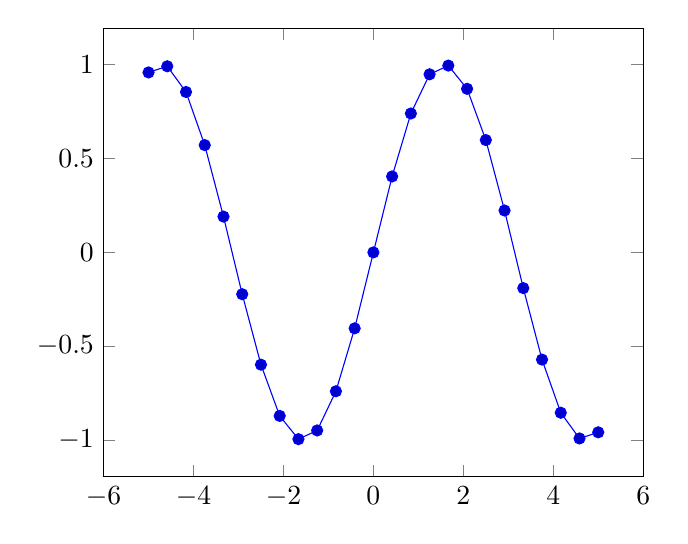
\begin{tikzpicture}
\begin{axis}
\addplot {sin(deg(x))};
\end{axis}
\end{tikzpicture}
\begin{tikzpicture}
\begin{axis}
\addplot+[only marks] {sin(deg(x))};
\end{axis}
\end{tikzpicture}

\vspace{24pt}
% \pgfplotsset{width=7cm,compat=1.9}
\begin{figure}
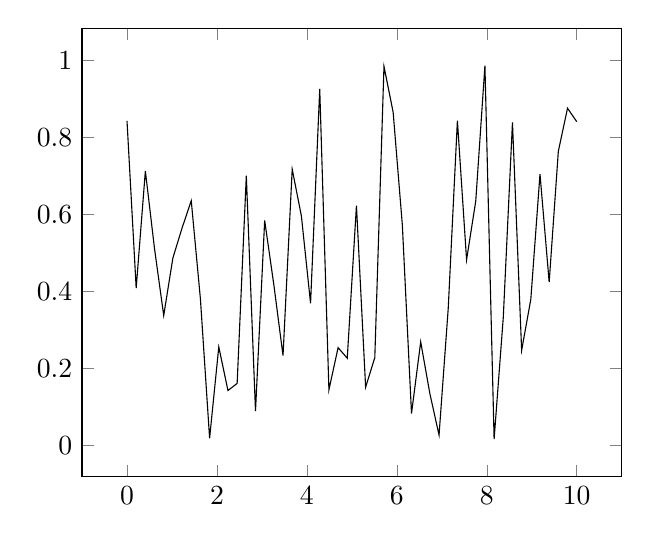
\begin{tikzpicture}
\begin{axis}
\addplot [domain=0:10,samples=50]{rnd};
\end{axis}
\end{tikzpicture}
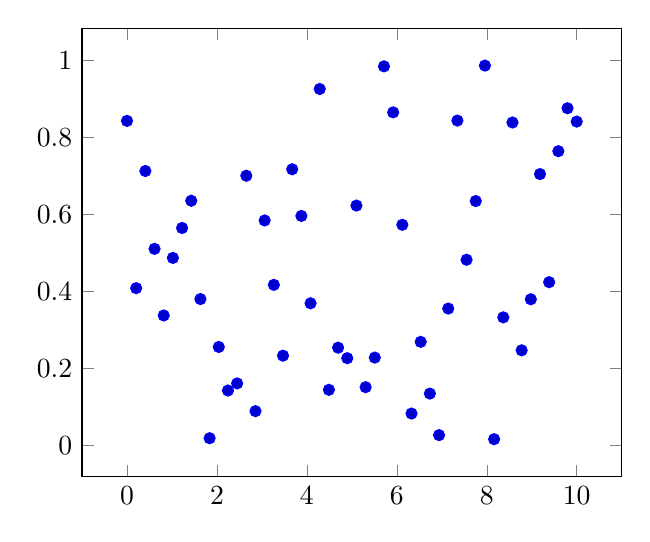
\begin{tikzpicture}
\begin{axis}
\addplot+[only marks,domain=0:10,samples=50] {rnd};
\end{axis}
\end{tikzpicture}
\caption{random data}
\end{figure}

\vspace{24pt}

% pdfplots manual p. 43
% Preamble: 
\pgfplotsset{width=6cm,compat=1.9}
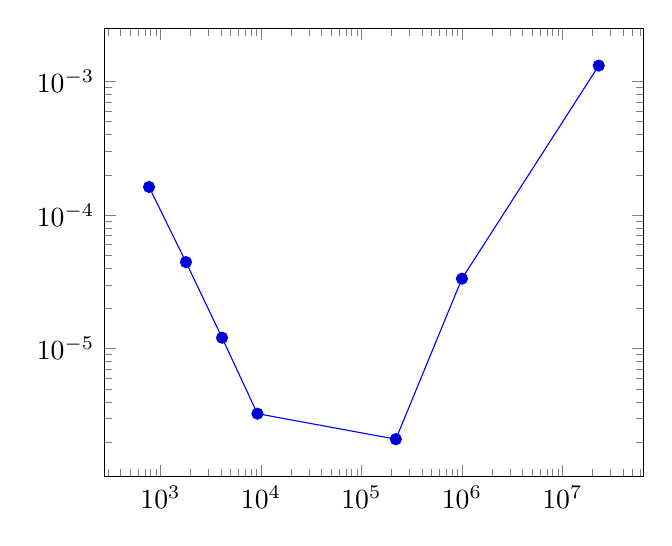
\begin{tikzpicture}
\begin{loglogaxis}
\addplot coordinates {
(769, 1.6227e-04)
(1793, 4.4425e-05)
(4097, 1.2071e-05)
(9217, 3.2610e-06)
(2.2e5, 2.1E-6)
(1e6, 0.00003341)
(2.3e7, 0.00131415)
};
\end{loglogaxis}
\end{tikzpicture}
\hspace{24pt}
\begin{tikzpicture}
\begin{semilogxaxis}
\addplot coordinates {
%% (769, 1.6227e-04)
(1793, 4.4425e-05)
(4097, 1.2071e-05)
(9217, 3.2610e-06)
(2.2e5, 2.1E-6)
%% (1e6, 0.00003341)
%% (2.3e7, 0.00131415)
};
\end{semilogxaxis}
\end{tikzpicture}

\vspace{24pt}
\begin{tikzpicture}
\begin{semilogxaxis}
\addplot coordinates {
%% (769, 1.6227e-04)
(1793, 4.4425)
(4097, 1.2071)
(9217, 3.2610)
(2.2e5, 2.1)
%% (1e6, 0.00003341)
%% (2.3e7, 0.00131415)
};
\end{semilogxaxis}
\end{tikzpicture}

\end{document}
